\documentclass[a4paper,11pt]{article}

\usepackage{../préambule}
\usetikzlibrary{positioning}

\newmdenv[style=redstyle]{attention}

\makeatletter
\renewcommand{\maketitle}{%
{\scriptsize colle dans ton cahier d'exercices, et écrit dans ton cahier} \vspace{0.5em}

	\begin{center}
		\LARGE
		\myuline{\@title}
	\end{center}
}
\makeatother

\title{Activité: proportionnalités}
\date{}
\author{}

\begin{document}

\maketitle

\begin{attention}[frametitle={Exercice 1}]
	On dispose de la figure suivante : \vspace{1em}

	\begin{center}
		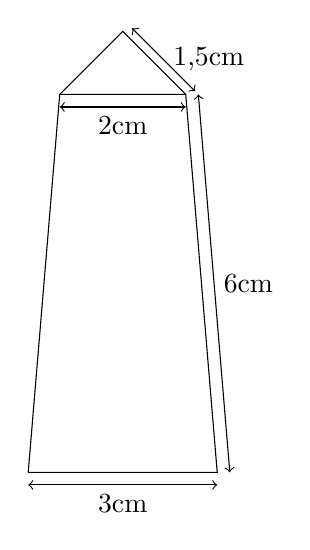
\begin{tikzpicture}[scale=0.8]
			\coordinate (A) at (0,0);
			\coordinate (B) at (3,0);
			\coordinate (C) at (2.5,6);
			\coordinate (D) at (0.5,6);
			\coordinate (E) at (1.5,7);

			\draw (A) -- (B) -- (C) -- (D) -- (A);
			\draw (C) -- (E) -- (D);

			\draw[<->] ([yshift=-0.2cm] A) -- node[anchor=north] {3cm} ([yshift=-0.2cm] B);
			\draw[<->] ([xshift=0.2cm] B) -- node[anchor=west] {6cm} ([xshift=0.2cm] C);
			\draw[<->] ([yshift=-0.2cm] D) -- node[anchor=north] {2cm} ([yshift=-0.2cm] C);
			\draw[<->] ([xshift=0.15cm,yshift=0.05cm] C) -- node[anchor=west] {1,5cm} ([xshift=0.15cm,yshift=0.05cm] E);
		\end{tikzpicture}
	\end{center}

	Reproduit cette figure dans ton cahier, \textbf{en faisant en sorte que la base de la tour fasse 5cm}.

	(Calcule les dimensions de la deuxième tour avant de dessiner, grâce à la proportionnalité !)
\end{attention}

\begin{attention}[frametitle={Exercice 2}]
	Une peintre veut faire de gigantesque toiles. Pour cela, elle fabrique elle-même ses couleurs, à partir de peinture \myuline{rouge}, \myuline{verte}, \myuline{bleue} et \myuline{noire}.

	La peintre a fourni les proportions de chaque couleur, ainsi que la quantité de noir : \vspace{1em}

	\renewcommand{\arraystretch}{1.2}
	\begin{tabular}{|c|c|c|c|c|c|c|}
		\hline
		                & Rouge   & Vert    & Bleu    & Noir    &  & Quantité de noir \\
		                & (en \%) & (en \%) & (en \%) & (en \%) &  & (en litres)      \\ \hline
		Fuschia         & 32      & 8       & 20      & 40      &  & 20               \\ \hline
		Or              & 33      & 22      & 0       & 45      &  & 15               \\ \hline
		Azur            & 4       & 17      & 26      & 53      &  & 26.5             \\ \hline
		Jaune           & 33      & 33      & 0       & 34      &  & 10               \\ \hline
		Argile          & 31      & 31      & 32      & 6       &  & 12               \\ \hline
		Indigo          & 16      & 4       & 32      & 48      &  & 12               \\ \hline
		Gris anthracite & 6       & 6       & 6       & 82      &  & 41               \\ \hline
	\end{tabular}
	\renewcommand{\arraystretch}{1}

	\begin{center}
		(⚠ Ce n'est pas un tableau de proportionnalité, juste un tableau normal !)
	\end{center}
	\vspace{0.5em}

	Pour chacune des couleurs demandées, calcule combien de litres de rouge, de vert, de bleu et de noir sont nécessaires.
\end{attention}

\end{document}